\documentclass{beamer}

\mode<presentation> {
	\usetheme{Madrid}
	%\setbeamertemplate{footline}
}

\usepackage{gensymb}
\usepackage[utf8]{inputenc}
\usepackage[russian]{babel}
\usepackage{graphicx} % Allows including images
\usepackage{booktabs} % Allows the use of \toprule, \midrule and \bottomrule in tables

\DeclareGraphicsExtensions{.jpg}

%----------------------------------------------------------------------------------------
%	Титульный лист
%----------------------------------------------------------------------------------------

\title{Leap Motion, карта глубин и OpenCV}

% \author{}
\institute[AIRLab]
{
	
\includegraphics[scale=0.15]{images/AIRLab_logo}
	\medskip
}
\date{}

%----------------------------------------------------------------------------------------
%	Презентация
%----------------------------------------------------------------------------------------

\begin{document}

	\begin{frame}
		\titlepage
	\end{frame}

	\begin{frame}
		\frametitle{Обзор}
		\tableofcontents
	\end{frame}

	\section{Leap Motion}
		\begin{frame}
			\frametitle{Leap Motion}
			
			\begin{center}
				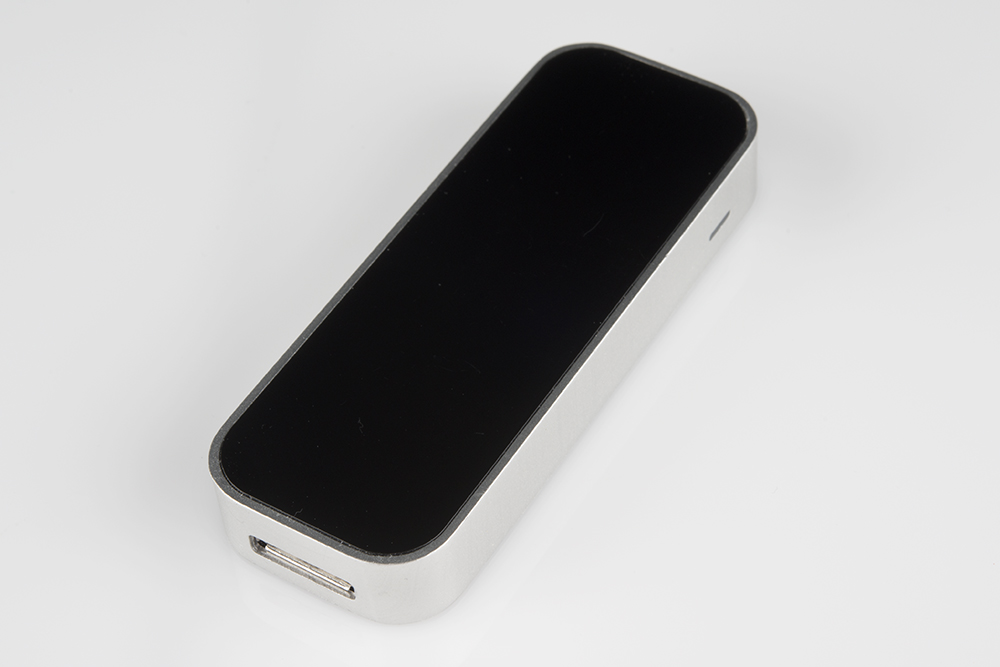
\includegraphics[scale=0.75]{images/LeapMotion}
			\end{center}
		\end{frame}
		
		\begin{frame}
			\frametitle{Особенности}
			
			\begin{itemize}
				\item 2 камеры с линзами fish-eye
				\item 3 инфракрасных светодиода
				\item Интерфейс: USB 3.0 micro-B
				\item Дальность распознавания объектов $\approx$ 60 см
				\item Угол обзора $\approx$ 135$\degree$
				\item Есть стандартный SDK, который периодически обновляется
				\item Монохромные изображения с разрешением 620x240 на выходе
			\end{itemize}
			
			\begin{center}
				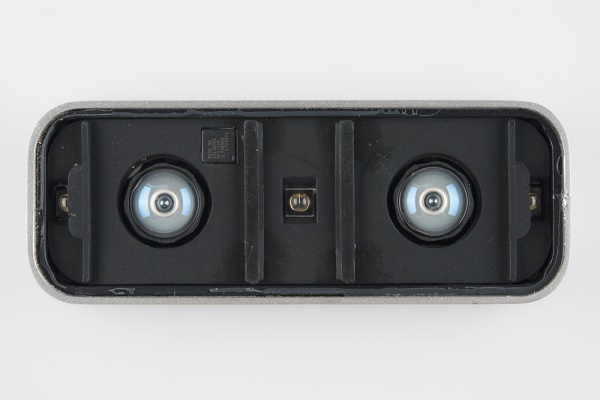
\includegraphics[scale=0.25]{images/LeapMotionDisassembled}
			\end{center}
		\end{frame}
		
		\begin{frame}
			\frametitle{Leap SDK}
			
			SDK позволяет делать множество интересных вещей:
			\begin{itemize}
				\item Определять руки, ладони, отдельные пальцы
				\item Определять инструменты (объекты цилиндрической формы - вытянутые и
					  тонкие)
				\item Определять жесты, такие как свайпы, нажатия и пр.
				\item Возвращать сырые изображения с камер
			\end{itemize}
		\end{frame}
		
		\begin{frame}
		    \frametitle{SGBM}
		   
		    \begin{center}
				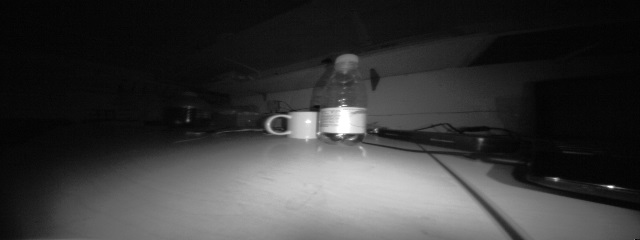
\includegraphics[scale=0.4]{images/raw0}
				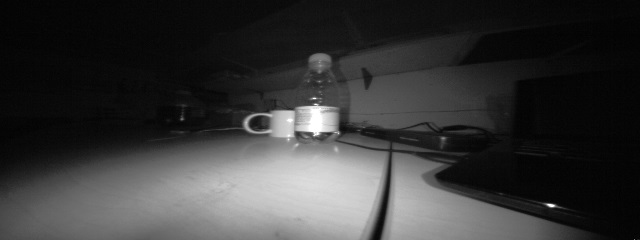
\includegraphics[scale=0.4]{images/raw1}
			\end{center}
		\end{frame}
		\begin{frame}
			\frametitle{Чем Leap Motion плох?}
			
			Цитата из интервью с одним из разработчиков:\\
			"... It’s very different from other things like the Kinect, and in
			normal device
			operation we have very different priorities than most other technologies.
			Our priority is precision, small movements, very low latency, very low CPU
			usage - so in order to do that we will often be making sacrifices that make
			what the device is doing completely not applicable to what I think you’re
			getting at, which is 3D scanning".
		\end{frame}
		
		\begin{frame}
			\frametitle{Чем Leap Motion плох?}
			
			\begin{itemize}
				\item Камеры очень чувствительны к освещению
				\item Отражения света от светодиодов распознаются как объекты
			\end{itemize}
		\end{frame}
		
	\section{Как мы творили темную магию объемного зрения}
		\begin{frame}
			\frametitle{Этапы}
			
			\begin{itemize}
				\item Калибровка
				\item Построение карты глубин (карты разностей/disparity map)
				\item Построение облака точек
				\item Blob detection
			\end{itemize}
		\end{frame}
		
		\begin{frame}
			\frametitle{Калибровка}
			
			В процессе производства камеры и линз всегда есть некоторые неточности,
			поэтому всегда, когда мы работаем со стереоскопией, существует необходимость
			в калибровке: нахождении внешних и внутренних параметров стереопары.
		\end{frame}

		\begin{frame}
			\frametitle{Калибровка}
			
			Ниже представлена модель проективной камеры
			\begin{equation}
			s
			\begin{bmatrix}
			u\\v\\1
			\end{bmatrix}
			=
			\begin{bmatrix}
			f_{x}&0&c_{x}\\
			0&f_{y}&c_{y}\\
			0&0&1
			\end{bmatrix}
			\begin{bmatrix}
			r_{11}&r_{11}&r_{11}&t_{1}\\
			r_{21}&r_{22}&r_{23}&t_{2}\\
			r_{31}&r_{32}&r_{33}&t_{3}
			\end{bmatrix}
			\begin{bmatrix}
			X\\Y\\Z\\1
			\end{bmatrix}
			\end{equation}
		\end{frame}
		
		\begin{frame}
			\frametitle{Внутренние параметры}
			
			\begin{center}
			$
			\begin{bmatrix}
			f_{x}&0&c_{x}\\
			0&f_{y}&c_{y}\\
			0&0&1
			\end{bmatrix}
			$
			\end{center}
			$(f_{x},f_{y})$ - фокусное расстояние\\
			$(c_{x},c_{y})$ - координаты принципальной точки 
			(точка пересечения плоскости изображения с оптической осью, совпадающая с
			центром фотографии. В реальных камерах, как правило, бывает немного смещена
			из-за оптических искажений)
		\end{frame}
				
		\begin{frame}
			\frametitle{Внешние параметры}
			
			\begin{center}
			$
			\begin{bmatrix}
			r_{11}&r_{11}&r_{11}&t_{1}\\
			r_{21}&r_{22}&r_{23}&t_{2}\\
			r_{31}&r_{32}&r_{33}&t_{3}
			\end{bmatrix}
			$
			\end{center}
			Матрица для перехода из ситемы координат мира в систему координат камеры
		\end{frame}
					
		\begin{frame}
			\frametitle{Другие переменные}
			
			$(X,Y,Z)$ - координаты исходной точки\\
			$(u,v)$ - координаты на изображении\\
			$s$ - переменная отвечающая за масштаб
		\end{frame}
		
		\begin{frame}
			\frametitle{Калибровка при помощи openCV}
			
			Один из стандартных способов для калибровки - использование изображения 
			шахматной доски.\\
			В OpenCV есть несколько стандартных функций для калибровки с использованием 
			шахматной доски и других шаблонов.
		\end{frame}
		
		\begin{frame}
		    \frametitle{Калибровка}
		   
		    \begin{center}
				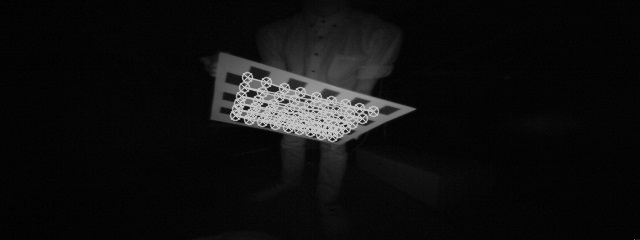
\includegraphics[scale=0.7]{images/leftCo2}
			\end{center}
		\end{frame}
		
		\begin{frame}
			\frametitle{Полученные данные}
			
			\begin{itemize}
				\item Матрицы камер - внутренние параметры камер
				\item Коэффициенты искажений для камер
				\item Матрицы для перехода между системами координат камер
				\item Матрицы связывающие точки между изображениями с разных камер
			\end{itemize}
		\end{frame}
		
		\begin{frame}
			\frametitle{Ректификация}
			
			Ректификация - процесс, необходимый для большинства алгоритмов поиска карты
			глубин. Он заключается в выполнении преобразования, при котором и правое, и
			левое изображения проецируются на плоскость, параллельную базовой линии
			(линии, соединяющей оптические центры камер). Тогда если $(x, y)$ - точка
			левой проекции, а $(x_{0},y_{0})$ - соответствующая ей точка правой проекции,
			то $y = y_{0}$.
		\end{frame}
		
		\begin{frame}
		    \frametitle{Изображения с камер}
		   
		    \begin{center}
				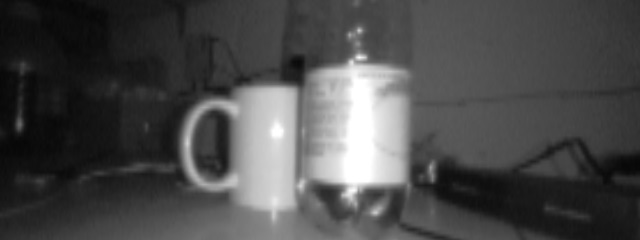
\includegraphics[scale=0.4]{images/rectL}
				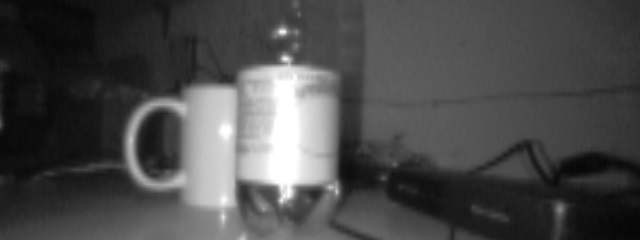
\includegraphics[scale=0.4]{images/rectR}
			\end{center}
		\end{frame}
		
		\begin{frame}
			\frametitle{Ректификация}
			
			Для ректификации применяются функции из библиотеки OpenCV.\\
			Сначала мы получаем матрицы для поворота систем координат камер, матрицы для
			перехода в новые системы координат и матрицу, которая позволит нам переходить
			от карты разностей к карте глубин.\\
			Затем работаем с конкретными изображениями.
		\end{frame}
		
		\begin{frame}
			\frametitle{Алгоритмы нахождения карт разностей в OpenCV}
			
			Существует несколько встроенных в OpenCV алгоритмов для нахождения разностных 
			карт:
			\begin{itemize}
				\item StereoBM - быстро (доли секунд), много шумов
				\item StereoSGBM - чуть медленней (все еще доли секунд), шумов меньше
				\item StereoVar - очень медленно(порядка ста секунд), карты разностей 	
					  близки к идеальным
			\end{itemize}	
			Для решения задачи был выбран алгоритм StereoSGBM.
		\end{frame}
		
		% TODO: дополнить описанием работы алгоритма
		\begin{frame}
			\frametitle{Описание алгоритма StereoSGBM}
			
			Получает на вход два изображения и некоторое количество параметров,
			возвращает карту разностей. Путем подбора волшебных чисел и написания
			утилиты, удобной для подбора коэффициентов, были получены результаты,
			содержащие минимально возможное количество шумов.
		\end{frame}
		
		\begin{frame}
		    \frametitle{SGBM}
		   
		    \begin{center}
				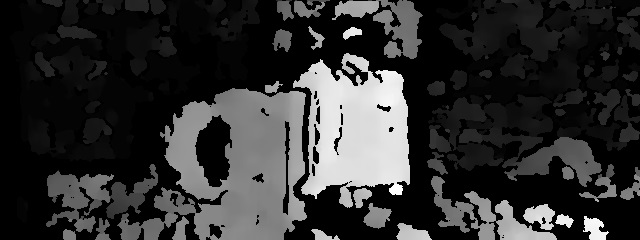
\includegraphics[scale=0.7]{images/disp}
			\end{center}
		\end{frame}
		
		\begin{frame}
		    \frametitle{SGBM with LUT}
		   
		    \begin{center}
				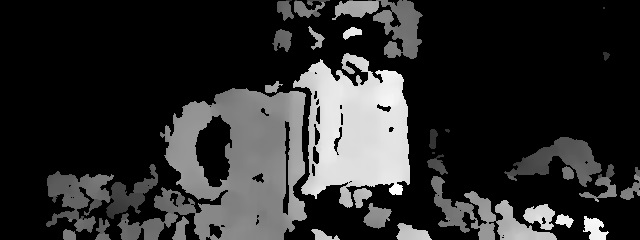
\includegraphics[scale=0.7]{images/dispLUT}
			\end{center}
		\end{frame}
		
		\begin{frame}
			\frametitle{Построение облака точек}
			
			Следующий этап - построить облако точек - это массив
			точек вида $(x, y, z)$ - координат относительно камеры, в
			этом помогают функции из библиотеки OpenCV.\\
			Затем запоминаются $z$-компоненты при разных расстояниях от камеры,
			и по полученным значениям интерполируем функцию зависимости
			расстояния до объекта от интенсивности цвета на карте глубин.
		\end{frame}
		
		\begin{frame}
			\frametitle{Blob detection}
			
			\textbf{Blob detection} - это нахождение регионов на изображении,
			которые отличаются по каким-то свойствам, вроде цвета
			или яркости, в сравнении с окружающими регионами.\\
			Грубо говоря, blob (капля) - это регион изображения,
			в котором какие-то свойства постоянны или почти
			постоянны.\\
			Все точки blob'а считаются в каком-то смысле
			одинаковыми.\\
		\end{frame}
		
		\begin{frame}
			\frametitle{Blob detection}
			
			Следующий этап - применить blob detection к карте глубин.\\
			С этой задачей вновь помог справиться OpenCV.\\
			Алгоритм, реализованный в OpenCV, таков:\\
			\begin{itemize}
				\item Конвертируем "бинарное" изображение - только
					  из черного и белого цветов по заданным извне границам
				\item Извлекаем компоненты связности
				\item Группируем центры компонент - близкие компоненты относятся к одному 
				      blob'у
				\item По полученным группам получаем результирующую позицию blob'а
			\end{itemize}
		\end{frame}

\end{document} 